\documentclass[twoside]{book}

% Packages required by doxygen
\usepackage{fixltx2e}
\usepackage{calc}
\usepackage{doxygen}
\usepackage[export]{adjustbox} % also loads graphicx
\usepackage{graphicx}
\usepackage[utf8]{inputenc}
\usepackage{makeidx}
\usepackage{multicol}
\usepackage{multirow}
\PassOptionsToPackage{warn}{textcomp}
\usepackage{textcomp}
\usepackage[nointegrals]{wasysym}
\usepackage[table]{xcolor}

% Font selection
\usepackage[T1]{fontenc}
\usepackage[scaled=.90]{helvet}
\usepackage{courier}
\usepackage{amssymb}
\usepackage{sectsty}
\renewcommand{\familydefault}{\sfdefault}
\allsectionsfont{%
  \fontseries{bc}\selectfont%
  \color{darkgray}%
}
\renewcommand{\DoxyLabelFont}{%
  \fontseries{bc}\selectfont%
  \color{darkgray}%
}
\newcommand{\+}{\discretionary{\mbox{\scriptsize$\hookleftarrow$}}{}{}}

% Page & text layout
\usepackage{geometry}
\geometry{%
  a4paper,%
  top=2.5cm,%
  bottom=2.5cm,%
  left=2.5cm,%
  right=2.5cm%
}
\tolerance=750
\hfuzz=15pt
\hbadness=750
\setlength{\emergencystretch}{15pt}
\setlength{\parindent}{0cm}
\setlength{\parskip}{3ex plus 2ex minus 2ex}
\makeatletter
\renewcommand{\paragraph}{%
  \@startsection{paragraph}{4}{0ex}{-1.0ex}{1.0ex}{%
    \normalfont\normalsize\bfseries\SS@parafont%
  }%
}
\renewcommand{\subparagraph}{%
  \@startsection{subparagraph}{5}{0ex}{-1.0ex}{1.0ex}{%
    \normalfont\normalsize\bfseries\SS@subparafont%
  }%
}
\makeatother

% Headers & footers
\usepackage{fancyhdr}
\pagestyle{fancyplain}
\fancyhead[LE]{\fancyplain{}{\bfseries\thepage}}
\fancyhead[CE]{\fancyplain{}{}}
\fancyhead[RE]{\fancyplain{}{\bfseries\leftmark}}
\fancyhead[LO]{\fancyplain{}{\bfseries\rightmark}}
\fancyhead[CO]{\fancyplain{}{}}
\fancyhead[RO]{\fancyplain{}{\bfseries\thepage}}
\fancyfoot[LE]{\fancyplain{}{}}
\fancyfoot[CE]{\fancyplain{}{}}
\fancyfoot[RE]{\fancyplain{}{\bfseries\scriptsize Generated by Doxygen }}
\fancyfoot[LO]{\fancyplain{}{\bfseries\scriptsize Generated by Doxygen }}
\fancyfoot[CO]{\fancyplain{}{}}
\fancyfoot[RO]{\fancyplain{}{}}
\renewcommand{\footrulewidth}{0.4pt}
\renewcommand{\chaptermark}[1]{%
  \markboth{#1}{}%
}
\renewcommand{\sectionmark}[1]{%
  \markright{\thesection\ #1}%
}

% Indices & bibliography
\usepackage{natbib}
\usepackage[titles]{tocloft}
\setcounter{tocdepth}{3}
\setcounter{secnumdepth}{5}
\makeindex

% Hyperlinks (required, but should be loaded last)
\usepackage{ifpdf}
\ifpdf
  \usepackage[pdftex,pagebackref=true]{hyperref}
\else
  \usepackage[ps2pdf,pagebackref=true]{hyperref}
\fi
\hypersetup{%
  colorlinks=true,%
  linkcolor=blue,%
  citecolor=blue,%
  unicode%
}

% Custom commands
\newcommand{\clearemptydoublepage}{%
  \newpage{\pagestyle{empty}\cleardoublepage}%
}

\usepackage{caption}
\captionsetup{labelsep=space,justification=centering,font={bf},singlelinecheck=off,skip=4pt,position=top}

%===== C O N T E N T S =====

\begin{document}

% Titlepage & ToC
\hypersetup{pageanchor=false,
             bookmarksnumbered=true,
             pdfencoding=unicode
            }
\pagenumbering{alph}
\begin{titlepage}
\vspace*{7cm}
\begin{center}%
{\Large Simulation }\\
\vspace*{1cm}
{\large Generated by Doxygen 1.8.14}\\
\end{center}
\end{titlepage}
\clearemptydoublepage
\pagenumbering{roman}
\tableofcontents
\clearemptydoublepage
\pagenumbering{arabic}
\hypersetup{pageanchor=true}

%--- Begin generated contents ---
\chapter{Hierarchical Index}
\section{Class Hierarchy}
This inheritance list is sorted roughly, but not completely, alphabetically\+:\begin{DoxyCompactList}
\item \contentsline{section}{Evaluator\+Of\+Scheduler}{\pageref{class_evaluator_of_scheduler}}{}
\item \contentsline{section}{Input}{\pageref{class_input}}{}
\item \contentsline{section}{Job}{\pageref{class_job}}{}
\item \contentsline{section}{Job\+Queue}{\pageref{class_job_queue}}{}
\begin{DoxyCompactList}
\item \contentsline{section}{Huge\+Job\+Queue}{\pageref{class_huge_job_queue}}{}
\item \contentsline{section}{Large\+Job\+Queue}{\pageref{class_large_job_queue}}{}
\item \contentsline{section}{Medium\+Job\+Queue}{\pageref{class_medium_job_queue}}{}
\item \contentsline{section}{Short\+Job\+Queue}{\pageref{class_short_job_queue}}{}
\end{DoxyCompactList}
\item \contentsline{section}{Node}{\pageref{class_node}}{}
\item \contentsline{section}{Output}{\pageref{class_output}}{}
\item \contentsline{section}{Scheduler}{\pageref{class_scheduler}}{}
\item \contentsline{section}{Test}{\pageref{class_test}}{}
\item \contentsline{section}{User}{\pageref{class_user}}{}
\begin{DoxyCompactList}
\item \contentsline{section}{I\+T\+Staff}{\pageref{class_i_t_staff}}{}
\item \contentsline{section}{Researcher}{\pageref{class_researcher}}{}
\item \contentsline{section}{Student}{\pageref{class_student}}{}
\end{DoxyCompactList}
\item \contentsline{section}{Users\+Generator}{\pageref{class_users_generator}}{}
\end{DoxyCompactList}

\chapter{Class Index}
\section{Class List}
Here are the classes, structs, unions and interfaces with brief descriptions\+:\begin{DoxyCompactList}
\item\contentsline{section}{\mbox{\hyperlink{class_evaluator_of_scheduler}{Evaluator\+Of\+Scheduler}} }{\pageref{class_evaluator_of_scheduler}}{}
\item\contentsline{section}{\mbox{\hyperlink{class_huge_job_queue}{Huge\+Job\+Queue}} }{\pageref{class_huge_job_queue}}{}
\item\contentsline{section}{\mbox{\hyperlink{class_input}{Input}} }{\pageref{class_input}}{}
\item\contentsline{section}{\mbox{\hyperlink{class_i_t_staff}{I\+T\+Staff}} }{\pageref{class_i_t_staff}}{}
\item\contentsline{section}{\mbox{\hyperlink{class_job}{Job}} }{\pageref{class_job}}{}
\item\contentsline{section}{\mbox{\hyperlink{class_job_queue}{Job\+Queue}} }{\pageref{class_job_queue}}{}
\item\contentsline{section}{\mbox{\hyperlink{class_large_job_queue}{Large\+Job\+Queue}} }{\pageref{class_large_job_queue}}{}
\item\contentsline{section}{\mbox{\hyperlink{class_medium_job_queue}{Medium\+Job\+Queue}} }{\pageref{class_medium_job_queue}}{}
\item\contentsline{section}{\mbox{\hyperlink{class_node}{Node}} }{\pageref{class_node}}{}
\item\contentsline{section}{\mbox{\hyperlink{class_output}{Output}} }{\pageref{class_output}}{}
\item\contentsline{section}{\mbox{\hyperlink{class_researcher}{Researcher}} }{\pageref{class_researcher}}{}
\item\contentsline{section}{\mbox{\hyperlink{class_scheduler}{Scheduler}} }{\pageref{class_scheduler}}{}
\item\contentsline{section}{\mbox{\hyperlink{class_short_job_queue}{Short\+Job\+Queue}} }{\pageref{class_short_job_queue}}{}
\item\contentsline{section}{\mbox{\hyperlink{class_student}{Student}} }{\pageref{class_student}}{}
\item\contentsline{section}{\mbox{\hyperlink{class_test}{Test}} }{\pageref{class_test}}{}
\item\contentsline{section}{\mbox{\hyperlink{class_user}{User}} }{\pageref{class_user}}{}
\item\contentsline{section}{\mbox{\hyperlink{class_users_generator}{Users\+Generator}} }{\pageref{class_users_generator}}{}
\end{DoxyCompactList}

\chapter{Class Documentation}
\hypertarget{class_evaluator_of_scheduler}{}\section{Evaluator\+Of\+Scheduler Class Reference}
\label{class_evaluator_of_scheduler}\index{Evaluator\+Of\+Scheduler@{Evaluator\+Of\+Scheduler}}
\subsection*{Public Member Functions}
\begin{DoxyCompactItemize}
\item 
\mbox{\Hypertarget{class_evaluator_of_scheduler_a0a1a38f0808b9cbc60af59cb1468f866}\label{class_evaluator_of_scheduler_a0a1a38f0808b9cbc60af59cb1468f866}} 
double {\bfseries evaluation} ()
\end{DoxyCompactItemize}


The documentation for this class was generated from the following files\+:\begin{DoxyCompactItemize}
\item 
D\+:/\+Cranfield work/\+Requirements Analysis and System Design/simulator project/\+Source\+Code/Evaluator\+Of\+Scheduler.\+h\item 
D\+:/\+Cranfield work/\+Requirements Analysis and System Design/simulator project/\+Source\+Code/Evaluator\+Of\+Scheduler.\+cpp\end{DoxyCompactItemize}

\hypertarget{class_huge_job_queue}{}\section{Huge\+Job\+Queue Class Reference}
\label{class_huge_job_queue}\index{Huge\+Job\+Queue@{Huge\+Job\+Queue}}
Inheritance diagram for Huge\+Job\+Queue\+:\begin{figure}[H]
\begin{center}
\leavevmode
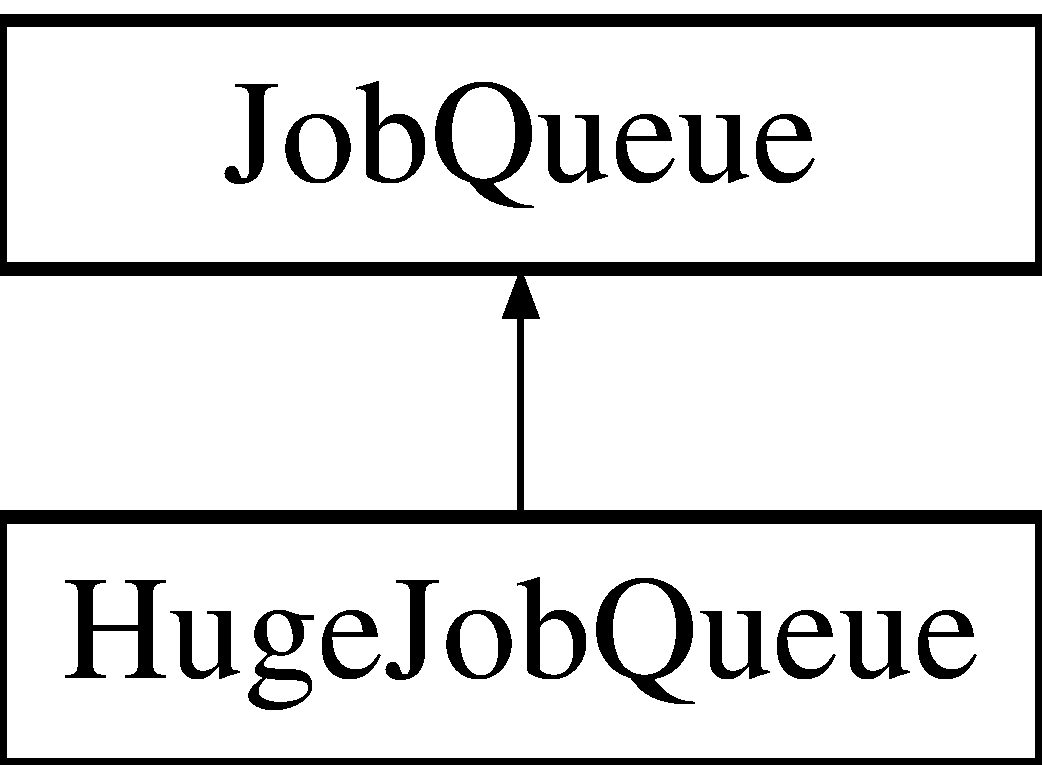
\includegraphics[height=2.000000cm]{class_huge_job_queue}
\end{center}
\end{figure}
\subsection*{Additional Inherited Members}


The documentation for this class was generated from the following files\+:\begin{DoxyCompactItemize}
\item 
D\+:/\+Cranfield work/\+Requirements Analysis and System Design/simulator project/\+Source\+Code/Huge\+Job\+Queue.\+h\item 
D\+:/\+Cranfield work/\+Requirements Analysis and System Design/simulator project/\+Source\+Code/Huge\+Job\+Queue.\+cpp\end{DoxyCompactItemize}

\hypertarget{class_input}{}\section{Input Class Reference}
\label{class_input}\index{Input@{Input}}
\subsection*{Public Member Functions}
\begin{DoxyCompactItemize}
\item 
\mbox{\Hypertarget{class_input_a1ee522db7c8b3cc5507e62d057ca5752}\label{class_input_a1ee522db7c8b3cc5507e62d057ca5752}} 
void {\bfseries time\+Step} (int time, \mbox{\hyperlink{class_users_generator}{Users\+Generator}} \&ug, \mbox{\hyperlink{class_scheduler}{Scheduler}} \&sch, \mbox{\hyperlink{class_node}{Node}} \&node)
\item 
\mbox{\Hypertarget{class_input_a12350cbbc8bcdcaf38bfc3562b7f4a97}\label{class_input_a12350cbbc8bcdcaf38bfc3562b7f4a97}} 
void {\bfseries start\+Jobs\+In\+Job\+Queue} (int time, \mbox{\hyperlink{class_users_generator}{Users\+Generator}} \&ug, \mbox{\hyperlink{class_scheduler}{Scheduler}} \&sch, \mbox{\hyperlink{class_node}{Node}} \&node, \mbox{\hyperlink{class_job_queue}{Job\+Queue}} \&jq)
\item 
\mbox{\Hypertarget{class_input_a5572ea662861b5f294195782ad953bf1}\label{class_input_a5572ea662861b5f294195782ad953bf1}} 
int {\bfseries get\+Nb\+Of\+Nodes} (\mbox{\hyperlink{class_node}{Node}} \&node, \mbox{\hyperlink{class_job_queue}{Job\+Queue}} \&jq)
\item 
\mbox{\Hypertarget{class_input_af91640b0926d1c88baae2561c1aadc5f}\label{class_input_af91640b0926d1c88baae2561c1aadc5f}} 
int {\bfseries get\+Nb\+Of\+Hours} (int type\+Of\+Queue, \mbox{\hyperlink{class_job_queue}{Job\+Queue}} \&jq)
\item 
\mbox{\Hypertarget{class_input_afa75d3fd99706a00c2847a324fefcd92}\label{class_input_afa75d3fd99706a00c2847a324fefcd92}} 
int {\bfseries get\+Type\+Of\+Nodes} ()
\item 
\mbox{\Hypertarget{class_input_ad4c4aa38487074bee3503ee4b8b40ef8}\label{class_input_ad4c4aa38487074bee3503ee4b8b40ef8}} 
double {\bfseries generate\+Number\+From\+Exponential\+Distribution} (double lambda)
\item 
\mbox{\Hypertarget{class_input_a2773675737b827a2f55d482b06fbcfd1}\label{class_input_a2773675737b827a2f55d482b06fbcfd1}} 
void {\bfseries print\+Numbers\+From\+Exponential\+Distribution} (double lambda, int iterations)
\end{DoxyCompactItemize}


The documentation for this class was generated from the following files\+:\begin{DoxyCompactItemize}
\item 
D\+:/\+Cranfield work/\+Requirements Analysis and System Design/simulator project/\+Source\+Code/Input.\+h\item 
D\+:/\+Cranfield work/\+Requirements Analysis and System Design/simulator project/\+Source\+Code/Input.\+cpp\end{DoxyCompactItemize}

\hypertarget{class_i_t_staff}{}\section{I\+T\+Staff Class Reference}
\label{class_i_t_staff}\index{I\+T\+Staff@{I\+T\+Staff}}
Inheritance diagram for I\+T\+Staff\+:\begin{figure}[H]
\begin{center}
\leavevmode
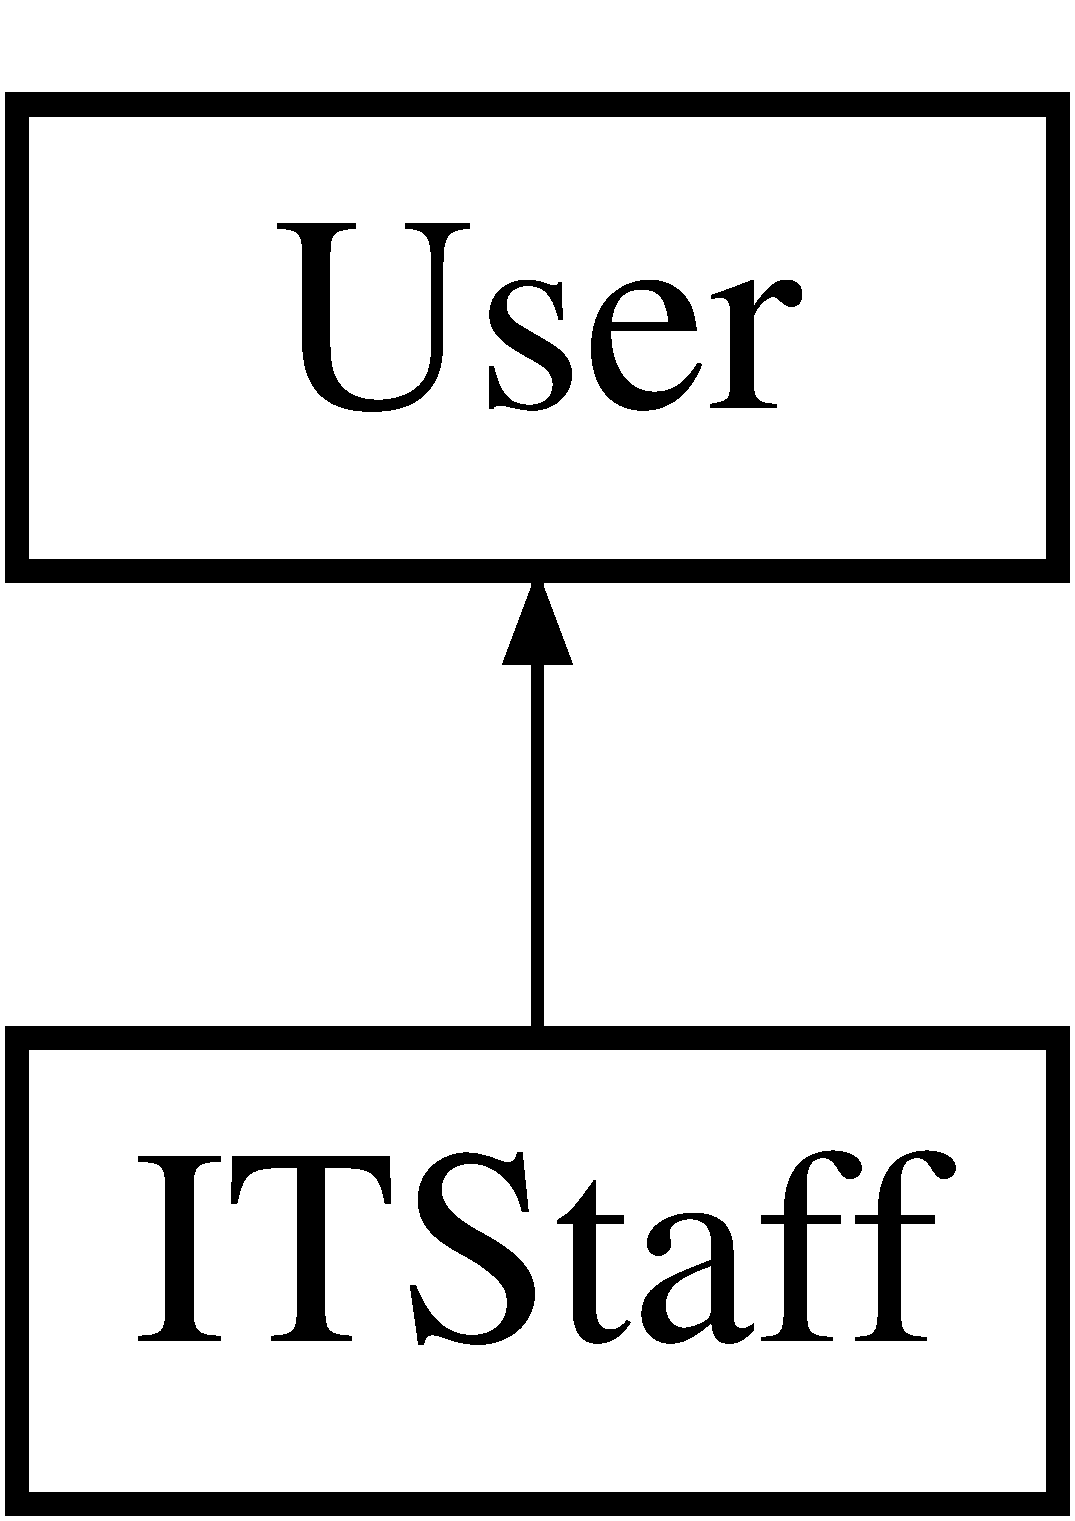
\includegraphics[height=2.000000cm]{class_i_t_staff}
\end{center}
\end{figure}
\subsection*{Public Member Functions}
\begin{DoxyCompactItemize}
\item 
\mbox{\Hypertarget{class_i_t_staff_a25ca02a72692ff5ed0c97f0c23415381}\label{class_i_t_staff_a25ca02a72692ff5ed0c97f0c23415381}} 
{\bfseries I\+T\+Staff} (int new\+Budget, int newid, double cap=1680.\+0)
\end{DoxyCompactItemize}


The documentation for this class was generated from the following files\+:\begin{DoxyCompactItemize}
\item 
D\+:/\+Cranfield work/\+Requirements Analysis and System Design/simulator project/\+Source\+Code/I\+T\+Staff.\+h\item 
D\+:/\+Cranfield work/\+Requirements Analysis and System Design/simulator project/\+Source\+Code/I\+T\+Staff.\+cpp\end{DoxyCompactItemize}

\hypertarget{class_job}{}\section{Job Class Reference}
\label{class_job}\index{Job@{Job}}
\subsection*{Public Member Functions}
\begin{DoxyCompactItemize}
\item 
\mbox{\Hypertarget{class_job_a47efbc618f9062b60684f79600d985d8}\label{class_job_a47efbc618f9062b60684f79600d985d8}} 
{\bfseries Job} (double job\+Budget, int nb\+Of\+Nodes, int nb\+Of\+Hours, int type\+Node, int user\+Id)
\end{DoxyCompactItemize}
\subsection*{Public Attributes}
\begin{DoxyCompactItemize}
\item 
\mbox{\Hypertarget{class_job_af31fad3ece1ef31d18d79435b8d002dc}\label{class_job_af31fad3ece1ef31d18d79435b8d002dc}} 
double {\bfseries budget}
\item 
\mbox{\Hypertarget{class_job_ae09a41715c749301bf627184d554a1d4}\label{class_job_ae09a41715c749301bf627184d554a1d4}} 
int {\bfseries nb\+Nodes}
\item 
\mbox{\Hypertarget{class_job_a6319e0142efd380b45893f719856823e}\label{class_job_a6319e0142efd380b45893f719856823e}} 
int {\bfseries nb\+Hours}
\item 
\mbox{\Hypertarget{class_job_a1aa451e277ebcc805a277dee15d34d44}\label{class_job_a1aa451e277ebcc805a277dee15d34d44}} 
int {\bfseries type\+Of\+Node}
\end{DoxyCompactItemize}


The documentation for this class was generated from the following files\+:\begin{DoxyCompactItemize}
\item 
D\+:/\+Cranfield work/\+Requirements Analysis and System Design/simulator project/\+Source\+Code/Job.\+h\item 
D\+:/\+Cranfield work/\+Requirements Analysis and System Design/simulator project/\+Source\+Code/Job.\+cpp\end{DoxyCompactItemize}

\hypertarget{class_job_queue}{}\section{Job\+Queue Class Reference}
\label{class_job_queue}\index{Job\+Queue@{Job\+Queue}}
Inheritance diagram for Job\+Queue\+:\begin{figure}[H]
\begin{center}
\leavevmode
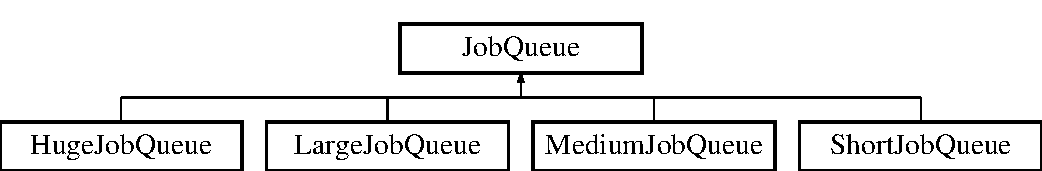
\includegraphics[height=2.000000cm]{class_job_queue}
\end{center}
\end{figure}
\subsection*{Public Member Functions}
\begin{DoxyCompactItemize}
\item 
\mbox{\Hypertarget{class_job_queue_a6d530bf47827ca5b7fd1733908206d9d}\label{class_job_queue_a6d530bf47827ca5b7fd1733908206d9d}} 
vector$<$ \mbox{\hyperlink{class_job}{Job}} $>$ {\bfseries get\+Job\+Queue} ()
\item 
\mbox{\Hypertarget{class_job_queue_aa21eaa87e05aca2ff536effe4fae1f36}\label{class_job_queue_aa21eaa87e05aca2ff536effe4fae1f36}} 
void {\bfseries add\+To\+Job\+Queue} (\mbox{\hyperlink{class_job}{Job}} job)
\item 
\mbox{\Hypertarget{class_job_queue_a40acca49c00bd568337e5e99cee2c936}\label{class_job_queue_a40acca49c00bd568337e5e99cee2c936}} 
void {\bfseries remove\+From\+Job\+Queue} (int i)
\item 
\mbox{\Hypertarget{class_job_queue_a337fbbcbcd9fdc0d7b4cdf1445540eeb}\label{class_job_queue_a337fbbcbcd9fdc0d7b4cdf1445540eeb}} 
void {\bfseries number\+Of\+Jobs\+Processed\+Plus1} ()
\item 
\mbox{\Hypertarget{class_job_queue_a82772a0000d5ad7380950c88c8718d01}\label{class_job_queue_a82772a0000d5ad7380950c88c8718d01}} 
void {\bfseries add\+New\+Wait\+Time} (int time\+Waited)
\item 
\mbox{\Hypertarget{class_job_queue_ad410dafe929327135889e271bd6a2d23}\label{class_job_queue_ad410dafe929327135889e271bd6a2d23}} 
void {\bfseries add\+New\+Run\+Time} (int time\+Run)
\item 
\mbox{\Hypertarget{class_job_queue_a38e08b929dda86f26a29c2c013905b74}\label{class_job_queue_a38e08b929dda86f26a29c2c013905b74}} 
double {\bfseries get\+Average\+Wait\+Time} ()
\item 
\mbox{\Hypertarget{class_job_queue_a3c386ff5559788ce23ee86dc2b69c93b}\label{class_job_queue_a3c386ff5559788ce23ee86dc2b69c93b}} 
double {\bfseries get\+Average\+Run\+Time} ()
\item 
\mbox{\Hypertarget{class_job_queue_a4965c12a271ee4cb1c9fadfcee2b51d3}\label{class_job_queue_a4965c12a271ee4cb1c9fadfcee2b51d3}} 
double {\bfseries get\+Average\+Turnaround\+Time\+Ratio} ()
\end{DoxyCompactItemize}
\subsection*{Public Attributes}
\begin{DoxyCompactItemize}
\item 
\mbox{\Hypertarget{class_job_queue_a2df2ae8313ca2248d59f68158fa64de5}\label{class_job_queue_a2df2ae8313ca2248d59f68158fa64de5}} 
vector$<$ \mbox{\hyperlink{class_job}{Job}} $>$ {\bfseries job\+Queue\+Vector}
\item 
\mbox{\Hypertarget{class_job_queue_abcf8363998ac230e81b6e84d13a0da05}\label{class_job_queue_abcf8363998ac230e81b6e84d13a0da05}} 
double {\bfseries cost\+Per\+Machine\+Hour}
\item 
\mbox{\Hypertarget{class_job_queue_aa14e93d8289f0cbffdd1e7fdb5991e00}\label{class_job_queue_aa14e93d8289f0cbffdd1e7fdb5991e00}} 
int {\bfseries max\+Nb\+Of\+Hours}
\item 
\mbox{\Hypertarget{class_job_queue_aec23b24c5671b66aeb8bcb619f390ab9}\label{class_job_queue_aec23b24c5671b66aeb8bcb619f390ab9}} 
int {\bfseries max\+Nb\+Of\+Nodes}
\item 
\mbox{\Hypertarget{class_job_queue_aee18b3b19b0faf073e1399a3725d92f7}\label{class_job_queue_aee18b3b19b0faf073e1399a3725d92f7}} 
int {\bfseries number\+Of\+Jobs\+Processed}
\item 
\mbox{\Hypertarget{class_job_queue_acc66a3f47ac7bbec772f0c5ea5d699c3}\label{class_job_queue_acc66a3f47ac7bbec772f0c5ea5d699c3}} 
vector$<$ int $>$ {\bfseries wait\+Time}
\item 
\mbox{\Hypertarget{class_job_queue_a3a9b97d1a3b1ee0da81747335a0a5d25}\label{class_job_queue_a3a9b97d1a3b1ee0da81747335a0a5d25}} 
vector$<$ int $>$ {\bfseries run\+Time}
\item 
\mbox{\Hypertarget{class_job_queue_ab6876a626f1767a5bb7e63a65ce1faef}\label{class_job_queue_ab6876a626f1767a5bb7e63a65ce1faef}} 
double {\bfseries lambda}
\item 
\mbox{\Hypertarget{class_job_queue_a2b9e866b703b97a2fcec2ef289a1f00a}\label{class_job_queue_a2b9e866b703b97a2fcec2ef289a1f00a}} 
int {\bfseries exponential\+Distribution\+Factor}
\end{DoxyCompactItemize}


The documentation for this class was generated from the following files\+:\begin{DoxyCompactItemize}
\item 
D\+:/\+Cranfield work/\+Requirements Analysis and System Design/simulator project/\+Source\+Code/Job\+Queue.\+h\item 
D\+:/\+Cranfield work/\+Requirements Analysis and System Design/simulator project/\+Source\+Code/Job\+Queue.\+cpp\end{DoxyCompactItemize}

\hypertarget{class_large_job_queue}{}\section{Large\+Job\+Queue Class Reference}
\label{class_large_job_queue}\index{Large\+Job\+Queue@{Large\+Job\+Queue}}
Inheritance diagram for Large\+Job\+Queue\+:\begin{figure}[H]
\begin{center}
\leavevmode
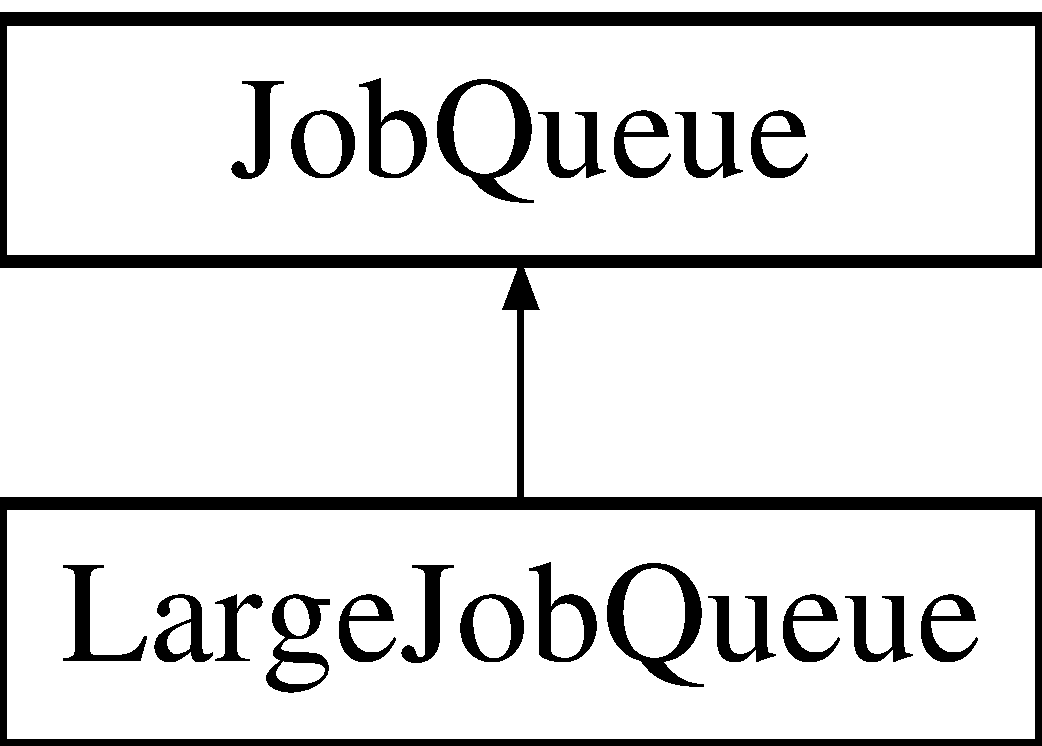
\includegraphics[height=2.000000cm]{class_large_job_queue}
\end{center}
\end{figure}
\subsection*{Additional Inherited Members}


The documentation for this class was generated from the following files\+:\begin{DoxyCompactItemize}
\item 
D\+:/\+Cranfield work/\+Requirements Analysis and System Design/simulator project/\+Source\+Code/Large\+Job\+Queue.\+h\item 
D\+:/\+Cranfield work/\+Requirements Analysis and System Design/simulator project/\+Source\+Code/Large\+Job\+Queue.\+cpp\end{DoxyCompactItemize}

\hypertarget{class_medium_job_queue}{}\section{Medium\+Job\+Queue Class Reference}
\label{class_medium_job_queue}\index{Medium\+Job\+Queue@{Medium\+Job\+Queue}}
Inheritance diagram for Medium\+Job\+Queue\+:\begin{figure}[H]
\begin{center}
\leavevmode
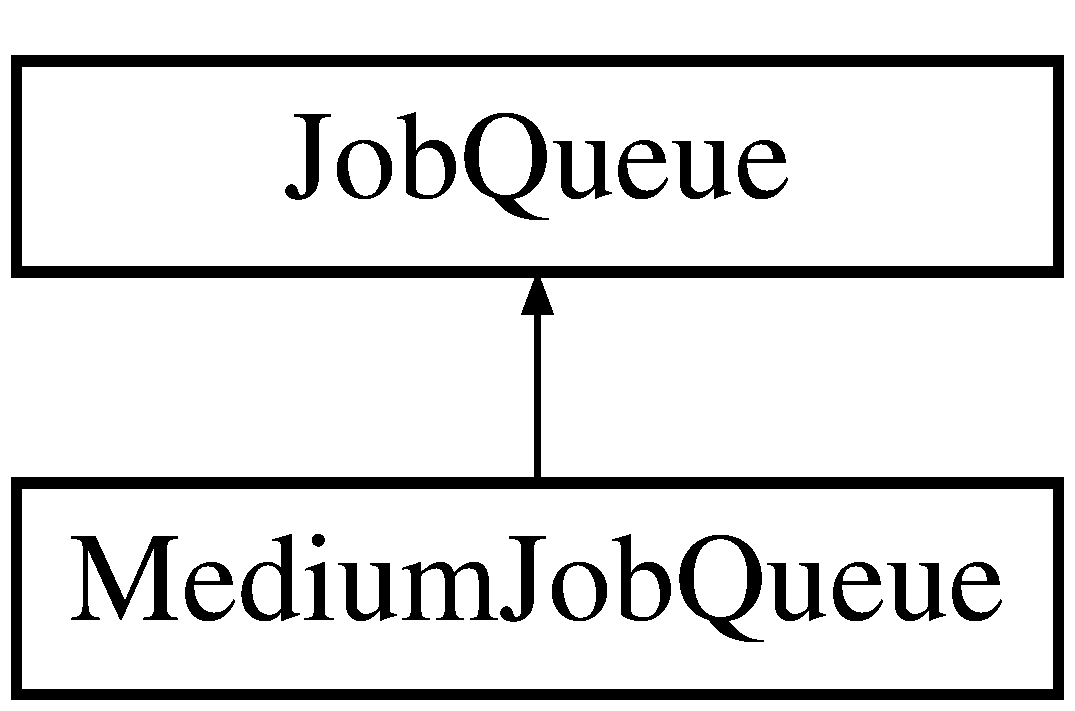
\includegraphics[height=2.000000cm]{class_medium_job_queue}
\end{center}
\end{figure}
\subsection*{Additional Inherited Members}


The documentation for this class was generated from the following files\+:\begin{DoxyCompactItemize}
\item 
D\+:/\+Cranfield work/\+Requirements Analysis and System Design/simulator project/\+Source\+Code/Medium\+Job\+Queue.\+h\item 
D\+:/\+Cranfield work/\+Requirements Analysis and System Design/simulator project/\+Source\+Code/Medium\+Job\+Queue.\+cpp\end{DoxyCompactItemize}

\hypertarget{class_node}{}\section{Node Class Reference}
\label{class_node}\index{Node@{Node}}
\subsection*{Public Member Functions}
\begin{DoxyCompactItemize}
\item 
\mbox{\Hypertarget{class_node_a9b392d27de54c97ef230c6f96975ec86}\label{class_node_a9b392d27de54c97ef230c6f96975ec86}} 
{\bfseries Node} (int nb\+Traditional\+Nodes=64, int nb\+Accelerated\+Nodes=32, int nb\+Specialized\+Nodes=32)
\item 
\mbox{\Hypertarget{class_node_a8ea7618f3d3c911f41befaf771c94c55}\label{class_node_a8ea7618f3d3c911f41befaf771c94c55}} 
void {\bfseries use\+Nodes} (Matrix \&nodes, int start\+Time, int nb\+Of\+Nodes, \mbox{\hyperlink{class_job_queue}{Job\+Queue}} \&job\+Queue)
\item 
\mbox{\Hypertarget{class_node_a429132bde9ec23913d9dfab4ffd23971}\label{class_node_a429132bde9ec23913d9dfab4ffd23971}} 
int {\bfseries get\+Total\+Number\+Of\+Machine\+Hours\+Consumed} ()
\end{DoxyCompactItemize}
\subsection*{Public Attributes}
\begin{DoxyCompactItemize}
\item 
\mbox{\Hypertarget{class_node_ab3c28d4dffc8911009b7af4b079ce99f}\label{class_node_ab3c28d4dffc8911009b7af4b079ce99f}} 
int {\bfseries nb\+Of\+Hours\+Per\+Week}
\item 
\mbox{\Hypertarget{class_node_a6bb2fba37331b31a5b57cba59ed34406}\label{class_node_a6bb2fba37331b31a5b57cba59ed34406}} 
int {\bfseries nb\+Of\+Traditional\+Nodes}
\item 
\mbox{\Hypertarget{class_node_a7065d23d72c9395a4c04462d70885c1b}\label{class_node_a7065d23d72c9395a4c04462d70885c1b}} 
int {\bfseries nb\+Of\+Accelerated\+Nodes}
\item 
\mbox{\Hypertarget{class_node_afb2cc27b3b3385f9d0bbc4f21a330841}\label{class_node_afb2cc27b3b3385f9d0bbc4f21a330841}} 
int {\bfseries nb\+Of\+Specialized\+Nodes}
\item 
\mbox{\Hypertarget{class_node_adeb696381aeabb3622f46ee44d0f5418}\label{class_node_adeb696381aeabb3622f46ee44d0f5418}} 
Matrix {\bfseries traditional\+Nodes}
\item 
\mbox{\Hypertarget{class_node_acfc5a971c0d55eebd3b9b487936263c6}\label{class_node_acfc5a971c0d55eebd3b9b487936263c6}} 
Matrix {\bfseries accelerated\+Nodes}
\item 
\mbox{\Hypertarget{class_node_ae46791f9ae6fbbaa5f16e4d6380b200d}\label{class_node_ae46791f9ae6fbbaa5f16e4d6380b200d}} 
Matrix {\bfseries specialized\+Nodes}
\end{DoxyCompactItemize}


The documentation for this class was generated from the following files\+:\begin{DoxyCompactItemize}
\item 
D\+:/\+Cranfield work/\+Requirements Analysis and System Design/simulator project/\+Source\+Code/Node.\+h\item 
D\+:/\+Cranfield work/\+Requirements Analysis and System Design/simulator project/\+Source\+Code/Node.\+cpp\end{DoxyCompactItemize}

\hypertarget{class_output}{}\section{Output Class Reference}
\label{class_output}\index{Output@{Output}}
\subsection*{Public Member Functions}
\begin{DoxyCompactItemize}
\item 
\mbox{\Hypertarget{class_output_acb9d8ee43f81560de2beec11bf8983bf}\label{class_output_acb9d8ee43f81560de2beec11bf8983bf}} 
void {\bfseries output\+Results\+Of\+The\+Simulation} (\mbox{\hyperlink{class_scheduler}{Scheduler}} \&sch, \mbox{\hyperlink{class_node}{Node}} \&node, \mbox{\hyperlink{class_users_generator}{Users\+Generator}} \&ug, int number\+Of\+Machine\+Hours\+Available, double operating\+Cost)
\item 
\mbox{\Hypertarget{class_output_a37b5da24dd73ba9c7fbc1d70807ee59a}\label{class_output_a37b5da24dd73ba9c7fbc1d70807ee59a}} 
void {\bfseries number\+Of\+Jobs\+Processed\+In\+Each\+Queue} (\mbox{\hyperlink{class_scheduler}{Scheduler}} \&sch)
\item 
\mbox{\Hypertarget{class_output_a17c8f535b597f35ae4756695aed70da4}\label{class_output_a17c8f535b597f35ae4756695aed70da4}} 
void {\bfseries actual\+Number\+Of\+Machine\+Hours\+Consumed\+By\+Each\+Job} (\mbox{\hyperlink{class_scheduler}{Scheduler}} \&sch)
\item 
\mbox{\Hypertarget{class_output_aeae2d017558edea58d43914e9601600c}\label{class_output_aeae2d017558edea58d43914e9601600c}} 
void {\bfseries utilization\+Ratio} (\mbox{\hyperlink{class_node}{Node}} \&node, int number\+Of\+Machine\+Hours\+Available)
\item 
\mbox{\Hypertarget{class_output_a0195b7d1a95f2a5d7ae4fc84f513ce58}\label{class_output_a0195b7d1a95f2a5d7ae4fc84f513ce58}} 
void {\bfseries price\+Paid\+By\+The\+Users} (\mbox{\hyperlink{class_users_generator}{Users\+Generator}} \&ug)
\item 
\mbox{\Hypertarget{class_output_a0d052cfab8080543ea59abf505523d27}\label{class_output_a0d052cfab8080543ea59abf505523d27}} 
void {\bfseries average\+Wait\+Time\+In\+Each\+Queue} (\mbox{\hyperlink{class_scheduler}{Scheduler}} \&sch)
\item 
\mbox{\Hypertarget{class_output_ac9a0aeeefa8ef13cf8849487ea0133be}\label{class_output_ac9a0aeeefa8ef13cf8849487ea0133be}} 
void {\bfseries average\+Turnaround\+Time\+Ratio} (\mbox{\hyperlink{class_scheduler}{Scheduler}} \&sch)
\item 
\mbox{\Hypertarget{class_output_a3adb2cfe1229a1267fe8160ab70c562e}\label{class_output_a3adb2cfe1229a1267fe8160ab70c562e}} 
void {\bfseries economic\+Balance\+Of\+The\+Centre} (\mbox{\hyperlink{class_users_generator}{Users\+Generator}} \&ug, double operating\+Cost)
\item 
\mbox{\Hypertarget{class_output_a536b72eb2ce4b4bc2b15b315e823be92}\label{class_output_a536b72eb2ce4b4bc2b15b315e823be92}} 
void {\bfseries show\+Traditional\+Nodes} (\mbox{\hyperlink{class_node}{Node}} \&node)
\item 
\mbox{\Hypertarget{class_output_a10c9b770f51f6809f8d1da04fa88aa2e}\label{class_output_a10c9b770f51f6809f8d1da04fa88aa2e}} 
void {\bfseries show\+Accelerated\+Nodes} (\mbox{\hyperlink{class_node}{Node}} \&node)
\item 
\mbox{\Hypertarget{class_output_a2e26fc88b8088a4cae12b7e6854992a6}\label{class_output_a2e26fc88b8088a4cae12b7e6854992a6}} 
void {\bfseries show\+Specialized\+Nodes} (\mbox{\hyperlink{class_node}{Node}} \&node)
\item 
\mbox{\Hypertarget{class_output_a063064bb29bc5b4de55705960785feff}\label{class_output_a063064bb29bc5b4de55705960785feff}} 
void {\bfseries show\+Nodes} (Matrix \&nodes)
\end{DoxyCompactItemize}


The documentation for this class was generated from the following files\+:\begin{DoxyCompactItemize}
\item 
D\+:/\+Cranfield work/\+Requirements Analysis and System Design/simulator project/\+Source\+Code/Output.\+h\item 
D\+:/\+Cranfield work/\+Requirements Analysis and System Design/simulator project/\+Source\+Code/Output.\+cpp\end{DoxyCompactItemize}

\hypertarget{class_researcher}{}\section{Researcher Class Reference}
\label{class_researcher}\index{Researcher@{Researcher}}
Inheritance diagram for Researcher\+:\begin{figure}[H]
\begin{center}
\leavevmode
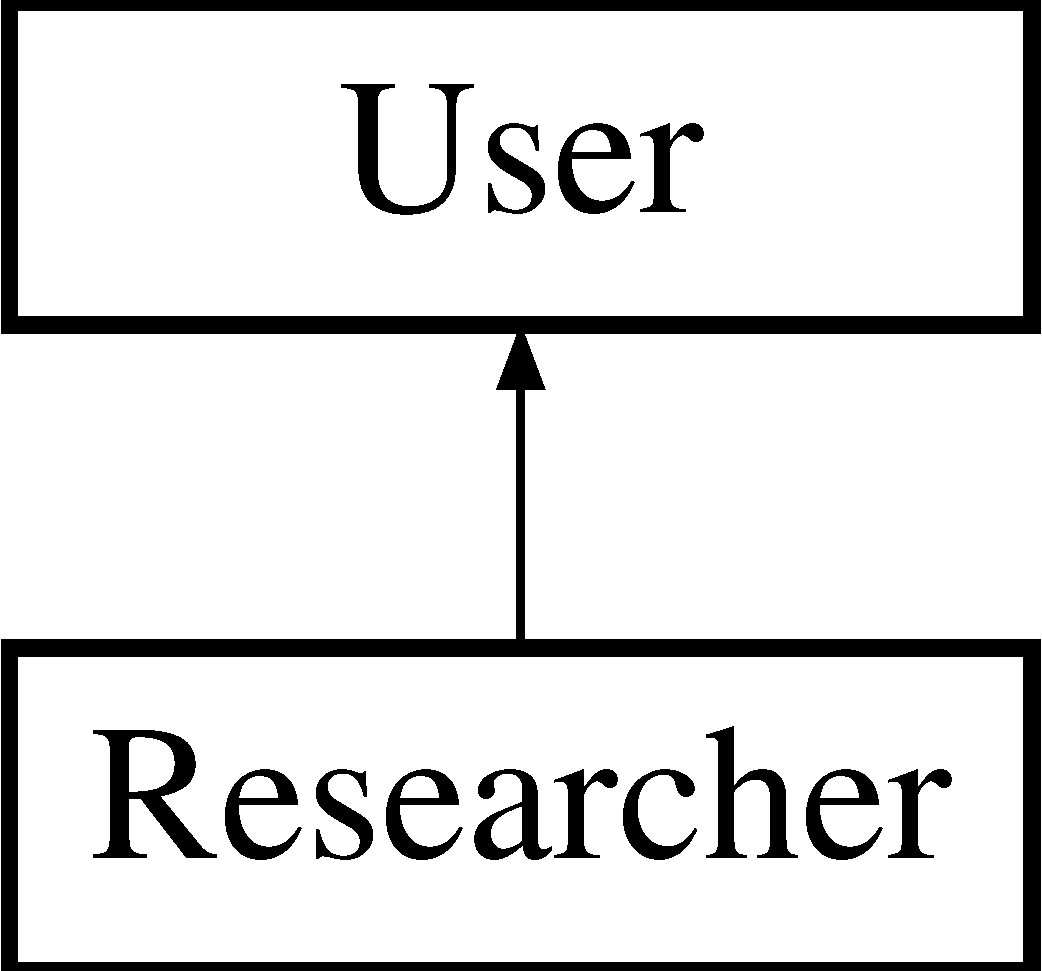
\includegraphics[height=2.000000cm]{class_researcher}
\end{center}
\end{figure}
\subsection*{Public Member Functions}
\begin{DoxyCompactItemize}
\item 
\mbox{\Hypertarget{class_researcher_a9c851cb4b8427bf22d4658df25ebcd02}\label{class_researcher_a9c851cb4b8427bf22d4658df25ebcd02}} 
{\bfseries Researcher} (int new\+Budget, int newid, double cap=1600.\+0)
\end{DoxyCompactItemize}


The documentation for this class was generated from the following files\+:\begin{DoxyCompactItemize}
\item 
D\+:/\+Cranfield work/\+Requirements Analysis and System Design/simulator project/\+Source\+Code/Researcher.\+h\item 
D\+:/\+Cranfield work/\+Requirements Analysis and System Design/simulator project/\+Source\+Code/Researcher.\+cpp\end{DoxyCompactItemize}

\hypertarget{class_scheduler}{}\section{Scheduler Class Reference}
\label{class_scheduler}\index{Scheduler@{Scheduler}}
\subsection*{Public Member Functions}
\begin{DoxyCompactItemize}
\item 
\mbox{\Hypertarget{class_scheduler_a9a97c1e371779013d1f391047831132b}\label{class_scheduler_a9a97c1e371779013d1f391047831132b}} 
void {\bfseries treat\+Job\+In\+Queue} (\mbox{\hyperlink{class_job_queue}{Job\+Queue}} \&job\+Queue, \mbox{\hyperlink{class_node}{Node}} \&node, int time)
\end{DoxyCompactItemize}
\subsection*{Public Attributes}
\begin{DoxyCompactItemize}
\item 
\mbox{\Hypertarget{class_scheduler_a230bcf2e686da11204241df858aee185}\label{class_scheduler_a230bcf2e686da11204241df858aee185}} 
\mbox{\hyperlink{class_short_job_queue}{Short\+Job\+Queue}} {\bfseries sjq}
\item 
\mbox{\Hypertarget{class_scheduler_a64b5c8f9d4801e0ce53b20a3915ba72a}\label{class_scheduler_a64b5c8f9d4801e0ce53b20a3915ba72a}} 
\mbox{\hyperlink{class_medium_job_queue}{Medium\+Job\+Queue}} {\bfseries mjq}
\item 
\mbox{\Hypertarget{class_scheduler_a235ae26896fab67995f166678bf0b506}\label{class_scheduler_a235ae26896fab67995f166678bf0b506}} 
\mbox{\hyperlink{class_large_job_queue}{Large\+Job\+Queue}} {\bfseries ljq}
\item 
\mbox{\Hypertarget{class_scheduler_a6f057765dd7084c1b0f37517eb90fcdb}\label{class_scheduler_a6f057765dd7084c1b0f37517eb90fcdb}} 
\mbox{\hyperlink{class_huge_job_queue}{Huge\+Job\+Queue}} {\bfseries hjq}
\item 
\mbox{\Hypertarget{class_scheduler_a14db1ba2a7ea1e676e75bd254e0418a4}\label{class_scheduler_a14db1ba2a7ea1e676e75bd254e0418a4}} 
vector$<$ int $>$ {\bfseries number\+Of\+Machine\+Hours\+Consumed}
\end{DoxyCompactItemize}


The documentation for this class was generated from the following files\+:\begin{DoxyCompactItemize}
\item 
D\+:/\+Cranfield work/\+Requirements Analysis and System Design/simulator project/\+Source\+Code/Scheduler.\+h\item 
D\+:/\+Cranfield work/\+Requirements Analysis and System Design/simulator project/\+Source\+Code/Scheduler.\+cpp\end{DoxyCompactItemize}

\hypertarget{class_short_job_queue}{}\section{Short\+Job\+Queue Class Reference}
\label{class_short_job_queue}\index{Short\+Job\+Queue@{Short\+Job\+Queue}}
Inheritance diagram for Short\+Job\+Queue\+:\begin{figure}[H]
\begin{center}
\leavevmode
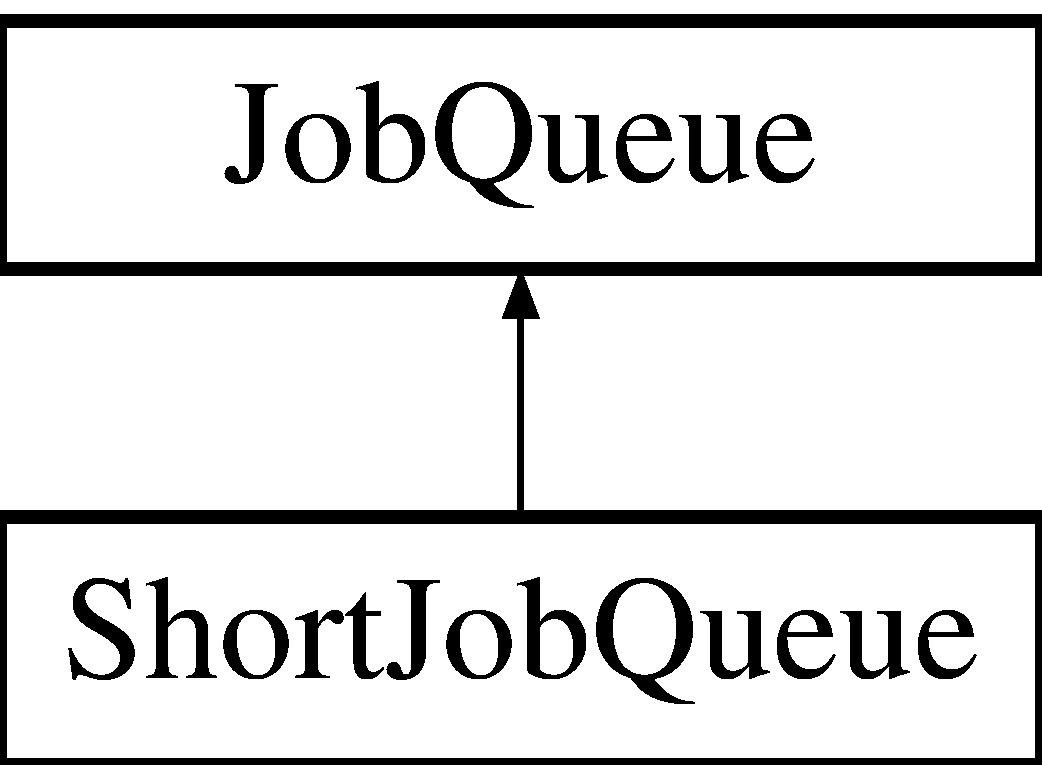
\includegraphics[height=2.000000cm]{class_short_job_queue}
\end{center}
\end{figure}
\subsection*{Additional Inherited Members}


The documentation for this class was generated from the following files\+:\begin{DoxyCompactItemize}
\item 
D\+:/\+Cranfield work/\+Requirements Analysis and System Design/simulator project/\+Source\+Code/Short\+Job\+Queue.\+h\item 
D\+:/\+Cranfield work/\+Requirements Analysis and System Design/simulator project/\+Source\+Code/Short\+Job\+Queue.\+cpp\end{DoxyCompactItemize}

\hypertarget{class_student}{}\section{Student Class Reference}
\label{class_student}\index{Student@{Student}}
Inheritance diagram for Student\+:\begin{figure}[H]
\begin{center}
\leavevmode
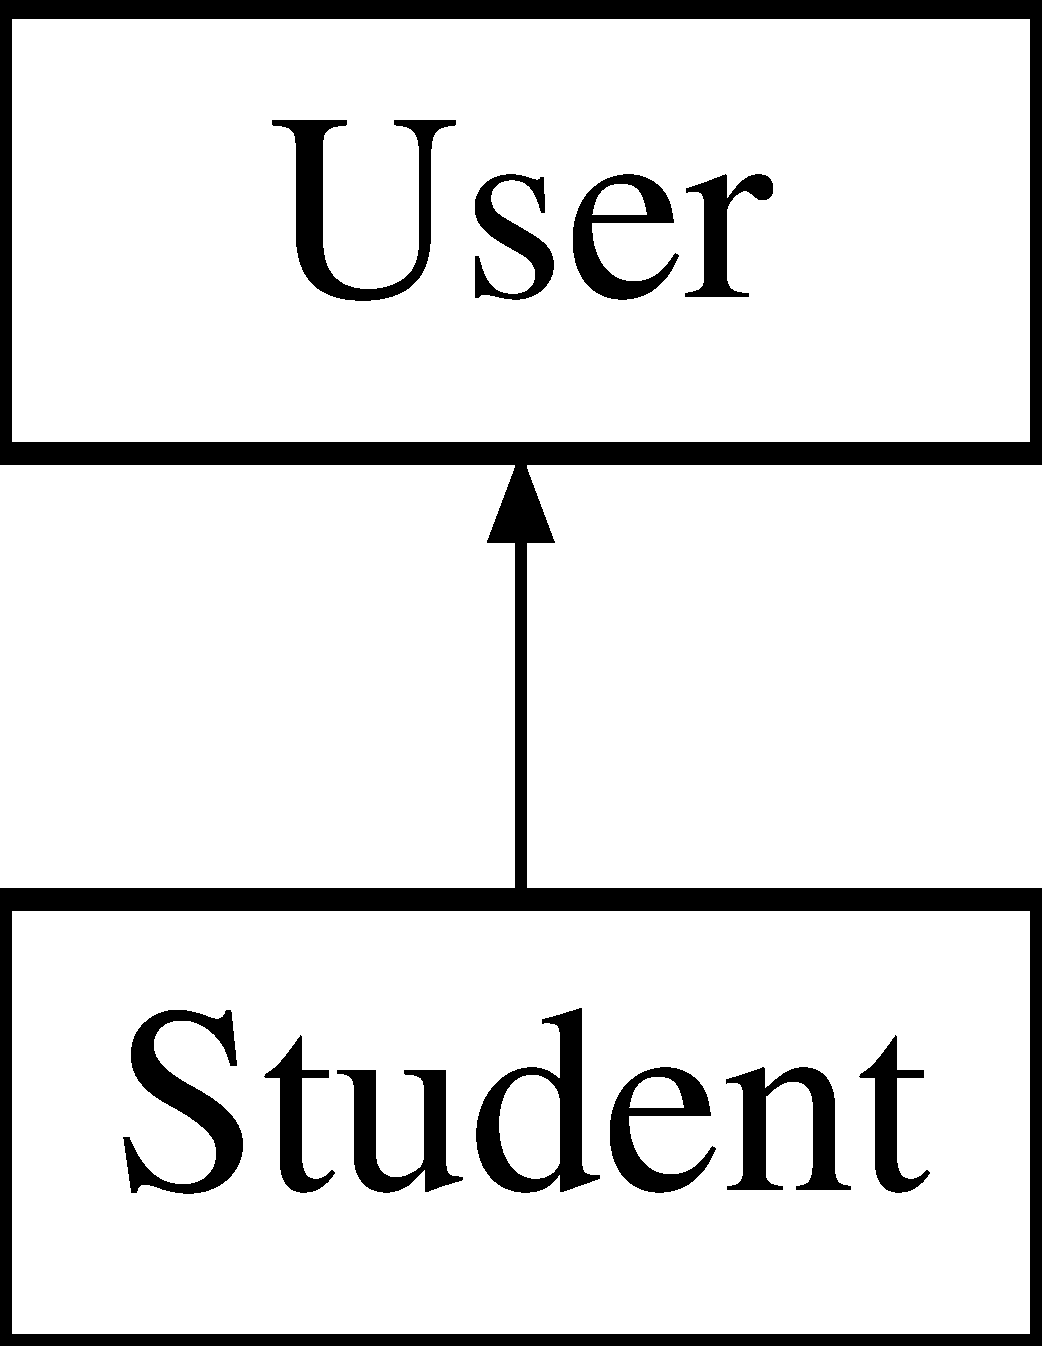
\includegraphics[height=2.000000cm]{class_student}
\end{center}
\end{figure}
\subsection*{Public Member Functions}
\begin{DoxyCompactItemize}
\item 
\mbox{\Hypertarget{class_student_a2d774a1d93be9037e9fcbda9750b9e33}\label{class_student_a2d774a1d93be9037e9fcbda9750b9e33}} 
{\bfseries Student} (int new\+Budget, int newid, double cap=100.\+0)
\end{DoxyCompactItemize}


The documentation for this class was generated from the following files\+:\begin{DoxyCompactItemize}
\item 
D\+:/\+Cranfield work/\+Requirements Analysis and System Design/simulator project/\+Source\+Code/Student.\+h\item 
D\+:/\+Cranfield work/\+Requirements Analysis and System Design/simulator project/\+Source\+Code/Student.\+cpp\end{DoxyCompactItemize}

\hypertarget{class_test}{}\section{Test Class Reference}
\label{class_test}\index{Test@{Test}}
\subsection*{Public Member Functions}
\begin{DoxyCompactItemize}
\item 
\mbox{\Hypertarget{class_test_a97d77dce48bd99f1af0a5c3a8be8b435}\label{class_test_a97d77dce48bd99f1af0a5c3a8be8b435}} 
void {\bfseries test\+Simulation} ()
\item 
\mbox{\Hypertarget{class_test_a4901403f34d65327a6fcb50b4b4387d3}\label{class_test_a4901403f34d65327a6fcb50b4b4387d3}} 
void {\bfseries test\+Input} ()
\item 
\mbox{\Hypertarget{class_test_a4a184aa153f2df4f4840fffed926cba5}\label{class_test_a4a184aa153f2df4f4840fffed926cba5}} 
void {\bfseries test\+Output} ()
\item 
\mbox{\Hypertarget{class_test_a0c0a7237b36e554b70393e9a9afb0827}\label{class_test_a0c0a7237b36e554b70393e9a9afb0827}} 
void {\bfseries test\+Job} ()
\item 
\mbox{\Hypertarget{class_test_a6c89d0a52d3737d13e7d7d559795f7f0}\label{class_test_a6c89d0a52d3737d13e7d7d559795f7f0}} 
void {\bfseries test\+Node} ()
\item 
\mbox{\Hypertarget{class_test_a153995343cf614c7196b3d64621ae62e}\label{class_test_a153995343cf614c7196b3d64621ae62e}} 
void {\bfseries test\+Scheduler} ()
\item 
\mbox{\Hypertarget{class_test_a9bd9be841180b6597b709bba9b057e90}\label{class_test_a9bd9be841180b6597b709bba9b057e90}} 
void {\bfseries test\+Users\+Generator} ()
\item 
\mbox{\Hypertarget{class_test_ae2a4a763ae3e91b6c4b3dc21eaa84e08}\label{class_test_ae2a4a763ae3e91b6c4b3dc21eaa84e08}} 
void {\bfseries test\+Evaluator\+Of\+Scheduler} ()
\item 
\mbox{\Hypertarget{class_test_a8ead44ebf288f773db2497712989286b}\label{class_test_a8ead44ebf288f773db2497712989286b}} 
void {\bfseries test\+Job\+Queue} ()
\item 
\mbox{\Hypertarget{class_test_ad556a698bd0eb5c9717d8c3e1143369b}\label{class_test_ad556a698bd0eb5c9717d8c3e1143369b}} 
void {\bfseries test\+Huge\+Job\+Queue} ()
\item 
\mbox{\Hypertarget{class_test_a139b768530114e54813d672dd0b88388}\label{class_test_a139b768530114e54813d672dd0b88388}} 
void {\bfseries test\+Large\+Job\+Queue} ()
\item 
\mbox{\Hypertarget{class_test_a8e49cb775161256e71bda76826cc3208}\label{class_test_a8e49cb775161256e71bda76826cc3208}} 
void {\bfseries test\+Medium\+Job\+Queue} ()
\item 
\mbox{\Hypertarget{class_test_abc29314e9cf9979de46392407b891220}\label{class_test_abc29314e9cf9979de46392407b891220}} 
void {\bfseries test\+Short\+Job\+Queue} ()
\item 
\mbox{\Hypertarget{class_test_a0e61f8c2dad4fdf5d60dd98a42c9f2a9}\label{class_test_a0e61f8c2dad4fdf5d60dd98a42c9f2a9}} 
void {\bfseries test\+User} ()
\item 
\mbox{\Hypertarget{class_test_a596b84b3a78ae1ed51f307c6641b3a3a}\label{class_test_a596b84b3a78ae1ed51f307c6641b3a3a}} 
void {\bfseries test\+I\+T\+Staff} ()
\item 
\mbox{\Hypertarget{class_test_a072c839b417675b9f34d4011e7d54147}\label{class_test_a072c839b417675b9f34d4011e7d54147}} 
void {\bfseries test\+Researcher} ()
\item 
\mbox{\Hypertarget{class_test_a44ed9c72e9610a1d492533445db23a5b}\label{class_test_a44ed9c72e9610a1d492533445db23a5b}} 
void {\bfseries test\+Student} ()
\end{DoxyCompactItemize}


The documentation for this class was generated from the following files\+:\begin{DoxyCompactItemize}
\item 
D\+:/\+Cranfield work/\+Requirements Analysis and System Design/simulator project/\+Source\+Code/Test.\+h\item 
D\+:/\+Cranfield work/\+Requirements Analysis and System Design/simulator project/\+Source\+Code/Test.\+cpp\end{DoxyCompactItemize}

\hypertarget{class_user}{}\section{User Class Reference}
\label{class_user}\index{User@{User}}
Inheritance diagram for User\+:\begin{figure}[H]
\begin{center}
\leavevmode
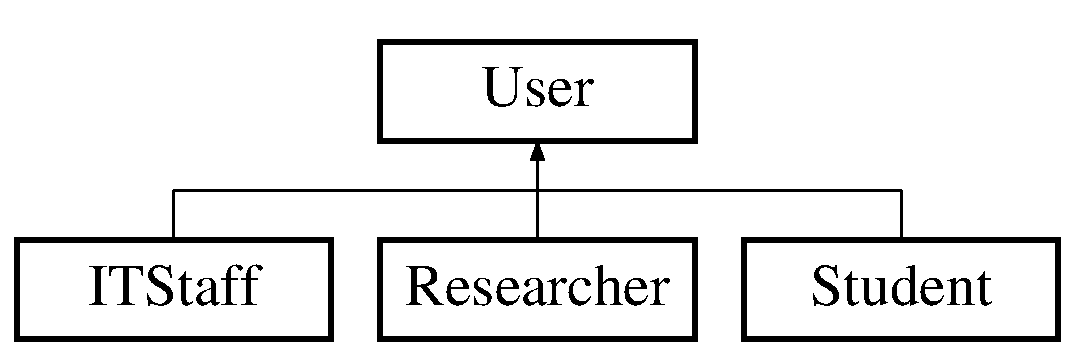
\includegraphics[height=2.000000cm]{class_user}
\end{center}
\end{figure}
\subsection*{Public Member Functions}
\begin{DoxyCompactItemize}
\item 
\mbox{\Hypertarget{class_user_ac5bc283639864f3d7f88ede4f0a8a332}\label{class_user_ac5bc283639864f3d7f88ede4f0a8a332}} 
{\bfseries User} (double user\+Budget, int user\+Id, double cap=1680.\+0)
\item 
\mbox{\Hypertarget{class_user_ae32aaa5d9ea260235599c9e4c4052046}\label{class_user_ae32aaa5d9ea260235599c9e4c4052046}} 
double {\bfseries get\+Budget} ()
\item 
\mbox{\Hypertarget{class_user_aec39d775c97e0c9f0234f45892d61f0d}\label{class_user_aec39d775c97e0c9f0234f45892d61f0d}} 
double {\bfseries get\+Budget\+Spent} ()
\item 
\mbox{\Hypertarget{class_user_a1e393732cd9838ab29445d9153333046}\label{class_user_a1e393732cd9838ab29445d9153333046}} 
int {\bfseries get\+Id} ()
\item 
\mbox{\Hypertarget{class_user_a792d82405cd2fd41f8e8b377d3f74827}\label{class_user_a792d82405cd2fd41f8e8b377d3f74827}} 
double {\bfseries get\+Instantaneous\+Cap} ()
\item 
\mbox{\Hypertarget{class_user_a842dee214d1c05758a362a5944b07cd1}\label{class_user_a842dee214d1c05758a362a5944b07cd1}} 
void {\bfseries spend\+Budget} (double budget\+User\+Spent)
\item 
\mbox{\Hypertarget{class_user_adcbf63de0acbc62bbb3c717e7652a91c}\label{class_user_adcbf63de0acbc62bbb3c717e7652a91c}} 
\mbox{\hyperlink{class_job}{Job}} {\bfseries create\+Job\+And\+Send\+Tosend\+Job\+To\+Job\+Queue} (int nb\+Of\+Nodes, int nb\+Of\+Hours, int type\+Node, \mbox{\hyperlink{class_job_queue}{Job\+Queue}} \&jobq, \mbox{\hyperlink{class_node}{Node}} \&node, int time, \mbox{\hyperlink{class_scheduler}{Scheduler}} \&sch)
\end{DoxyCompactItemize}
\subsection*{Private Attributes}
\begin{DoxyCompactItemize}
\item 
\mbox{\Hypertarget{class_user_a43dfb87a97cd57a69f2c6e56699c2148}\label{class_user_a43dfb87a97cd57a69f2c6e56699c2148}} 
double {\bfseries budget}
\item 
\mbox{\Hypertarget{class_user_a32e65c79e5f293afeaab91fa4f9e26ae}\label{class_user_a32e65c79e5f293afeaab91fa4f9e26ae}} 
double {\bfseries budget\+Spent}
\item 
\mbox{\Hypertarget{class_user_aa7e6e39b43020bbe9c3a196b3689b0f7}\label{class_user_aa7e6e39b43020bbe9c3a196b3689b0f7}} 
int {\bfseries id}
\item 
\mbox{\Hypertarget{class_user_adf08970f798ea619121d972dde81dad3}\label{class_user_adf08970f798ea619121d972dde81dad3}} 
double {\bfseries instantaneous\+Cap}
\end{DoxyCompactItemize}


The documentation for this class was generated from the following files\+:\begin{DoxyCompactItemize}
\item 
D\+:/\+Cranfield work/\+Requirements Analysis and System Design/simulator project/\+Source\+Code/User.\+h\item 
D\+:/\+Cranfield work/\+Requirements Analysis and System Design/simulator project/\+Source\+Code/User.\+cpp\end{DoxyCompactItemize}

\hypertarget{class_users_generator}{}\section{Users\+Generator Class Reference}
\label{class_users_generator}\index{Users\+Generator@{Users\+Generator}}
\subsection*{Public Member Functions}
\begin{DoxyCompactItemize}
\item 
\mbox{\Hypertarget{class_users_generator_aba9dc7527b95d02b466a9328bcfda268}\label{class_users_generator_aba9dc7527b95d02b466a9328bcfda268}} 
{\bfseries Users\+Generator} (int nb\+I\+T\+Staff, int nb\+Researchers, int nb\+Students, bool is\+Budget\+In\+Input)
\item 
\mbox{\Hypertarget{class_users_generator_a5d6afb5f6fea2830431eb39e56bfb904}\label{class_users_generator_a5d6afb5f6fea2830431eb39e56bfb904}} 
double {\bfseries get\+Budget\+I\+T\+Staff} ()
\item 
\mbox{\Hypertarget{class_users_generator_a5a6158b447c5c8b5bc48c771f127b893}\label{class_users_generator_a5a6158b447c5c8b5bc48c771f127b893}} 
double {\bfseries get\+Budget\+Researchers} ()
\item 
\mbox{\Hypertarget{class_users_generator_a42b91ad7272b8bb79a9f4aa5c3220480}\label{class_users_generator_a42b91ad7272b8bb79a9f4aa5c3220480}} 
double {\bfseries get\+Budget\+Students} ()
\item 
\mbox{\Hypertarget{class_users_generator_a90ed8eb2e6b3fd62abb97f5f4e1a6559}\label{class_users_generator_a90ed8eb2e6b3fd62abb97f5f4e1a6559}} 
double {\bfseries get\+Budget\+Spent\+I\+T\+Staff} ()
\item 
\mbox{\Hypertarget{class_users_generator_acea0ae4a4aa518a2db58e6dde2bf44ce}\label{class_users_generator_acea0ae4a4aa518a2db58e6dde2bf44ce}} 
double {\bfseries get\+Budget\+Spent\+Researchers} ()
\item 
\mbox{\Hypertarget{class_users_generator_ae6f2cb5583598a843029981d177a7c11}\label{class_users_generator_ae6f2cb5583598a843029981d177a7c11}} 
double {\bfseries get\+Budget\+Spent\+Students} ()
\end{DoxyCompactItemize}
\subsection*{Public Attributes}
\begin{DoxyCompactItemize}
\item 
\mbox{\Hypertarget{class_users_generator_a80b10f8dcb7620067a7075ed88ea2a45}\label{class_users_generator_a80b10f8dcb7620067a7075ed88ea2a45}} 
int {\bfseries nb\+Of\+I\+T\+Staff}
\item 
\mbox{\Hypertarget{class_users_generator_a259450d4f3b905f64ba6808c8a7a02f5}\label{class_users_generator_a259450d4f3b905f64ba6808c8a7a02f5}} 
int {\bfseries nb\+Of\+Researchers}
\item 
\mbox{\Hypertarget{class_users_generator_adee64bd85db36bc2843672655c63ae89}\label{class_users_generator_adee64bd85db36bc2843672655c63ae89}} 
int {\bfseries nb\+Of\+Students}
\item 
\mbox{\Hypertarget{class_users_generator_a4f1465aa85ef7f9df34d53ceb975d0ac}\label{class_users_generator_a4f1465aa85ef7f9df34d53ceb975d0ac}} 
vector$<$ \mbox{\hyperlink{class_i_t_staff}{I\+T\+Staff}} $>$ {\bfseries I\+T\+Staff\+List}
\item 
\mbox{\Hypertarget{class_users_generator_ad0f9f79843590cfb3cc184d13b978e5f}\label{class_users_generator_ad0f9f79843590cfb3cc184d13b978e5f}} 
vector$<$ \mbox{\hyperlink{class_researcher}{Researcher}} $>$ {\bfseries Researcher\+List}
\item 
\mbox{\Hypertarget{class_users_generator_a57ce948f6af95b98ec2fe3e629988217}\label{class_users_generator_a57ce948f6af95b98ec2fe3e629988217}} 
vector$<$ \mbox{\hyperlink{class_student}{Student}} $>$ {\bfseries Student\+List}
\end{DoxyCompactItemize}


The documentation for this class was generated from the following files\+:\begin{DoxyCompactItemize}
\item 
D\+:/\+Cranfield work/\+Requirements Analysis and System Design/simulator project/\+Source\+Code/Users\+Generator.\+h\item 
D\+:/\+Cranfield work/\+Requirements Analysis and System Design/simulator project/\+Source\+Code/Users\+Generator.\+cpp\end{DoxyCompactItemize}

%--- End generated contents ---

% Index
\backmatter
\newpage
\phantomsection
\clearemptydoublepage
\addcontentsline{toc}{chapter}{Index}
\printindex

\end{document}
